\section{gyakorlat (2025. november 12.)}
\subsection{"Sztringológia"}

Karaktersorozatok hasonlósága
\begin{itemize}[label=$\rightarrow$]
    \item Levenshtein távolság (optimális szekvenciaillesztés)
    \item leghosszabb közös részsorozat (LKR)
\end{itemize}
Mindkét esetben DP\\
$X = (x_1, x_2, \cdots, x_m)$ és $Y = (y_1, y_2, \cdots, y_n)$ $\rightarrow \mathcal{O}(mn)$


\subsubsection*{Leghosszabb közös részsorozat (LKR, előadáson "vázlatosan" volt)}
\setulcolor{black}
\textbf{Optimális részstruktúra tulajdonság}

$X_i = (x_1, x_2, \cdots, x_i)$ és $Y_j = (y_1, y_2, \cdots, y_j)$ prefixek LKR-jének meghatározása van éppen terítéken.

Tfh. $X_i$ és $Y_j$ egy LKR-je $Z_h = (z_1, z_2, \cdots, z_h)$

Ekkor\\
\textbf{(A)} Ha $x_i = y_j$, akkor $z_h = x_i = y_j$ és $Z' = (z_1, z_2, \cdots, z_{h-1})$ egy LKR $X_{i-1}$-hez és $Y_{j-1}$-hez.
A másik két esetben $x_i \neq y_j$, így biztosan $z_h \neq x_i$ vagy $z_h \neq y_j$.\\
\textbf{(B)} Ha $z_h \neq x_i$, akkor $Z$ egy LKR $x_{i-1}$-hez és $Y_j$-hez.\\
\textbf{(C)} Ha $z_h \neq y_j$, akkor $Z$ egy LKR $X_i$-hez és $y_{j-1}$-hez.

\textbf{Bizonyítás}\\
\textbf{(A)} Itt két állítás van!
Kezdjük azzal, hogy $z_h = x_i = y_j$.
Indirekt tfh. ez nem igaz, vagyis $z_h \neq x_i, y_j$.

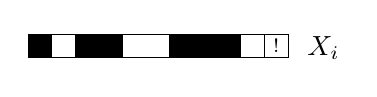
\begin{tikzpicture}[scale=0.3]
\draw(0,0) rectangle ++(11,1);
\draw[fill=black] (0,0) rectangle ++(1,1);
\draw[fill=black] (2,0) rectangle ++(1,1);
\draw[fill=black] (3,0) rectangle ++(1,1);
\draw[fill=black] (6,0) rectangle ++(1,1);
\draw[fill=black] (7,0) rectangle ++(1,1);
\draw[fill=black] (8,0) rectangle ++(1,1);
\draw (10,0) rectangle ++(1,1);
\node at (10.5, 0.5){\scriptsize !};

\node at (12.5, 0.4) {$X_i$};
\end{tikzpicture}

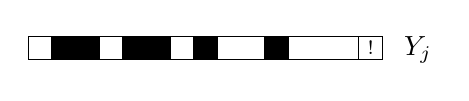
\begin{tikzpicture}[scale=0.3]
\draw(0,0) rectangle ++(15,1);
\draw[fill=black] (1,0) rectangle ++(1,1);
\draw[fill=black] (2,0) rectangle ++(1,1);
\draw[fill=black] (4,0) rectangle ++(1,1);
\draw[fill=black] (5,0) rectangle ++(1,1);
\draw[fill=black] (7,0) rectangle ++(1,1);
\draw[fill=black] (10,0) rectangle ++(1,1);
\draw (14,0) rectangle ++(1,1);
\node at (14.5, 0.5){\scriptsize !};

\node at (16.5, 0.4) {$Y_j$};
\end{tikzpicture}


\begin{tikzpicture}[scale=0.3]
\draw[fill=black] (0,0) rectangle ++(1,1);
\end{tikzpicture}
-k $\rightarrow Z$

Ám ekkor $Z$ biztos nem LKR $x_i$-hez és $Y_j$-hez, hiszen $Z$ végére írva az $x_i = y_j$ karaktert egy $Z$-nél hosszabb közös részsorozatát látjuk $X_i$-nek és $Y_j$-nek.

Ezek után jöjjön a második rész.
Most $Z'$ nyilván közös részsorozata $X_{i-1}$-nek és $Y_{j-1}$-nek.
Indirekt tfh. $Z'$ nem LKR $X_{i-1}$-hez és $Y_{j-1}$-hez, vagyis van olyan $Z'$-nél hosszabb $Z'$ sorozat, amely közös részsorozata $X_{i-1}$-nek és $Y_{j-1}$-nek.
Ha most $Z"$ végére írjuk az $x_i = y_j$ karaktert, az egy $Z$-nél hosszabb közös részsorozata lesz $X_i$-nek és $Y_j$-nek, \textbf{ellentmondás}.

\textbf{(B)} Most egyrészt $Z$ közös részsorozata $X_{i-1}$-nek és $Y_j$-nek, másrészt ha lenne egy $Z$-nél hosszabb közös részsorozata $X_{i-1}$-nek és $Y_j$-nek, az egy $Z$-nél hosszabb közös részsorozata lenne $X_i$-nek és $Y_j$-nek, ami nem lehet.

\textbf{(C)} analóg módon (B)-hez.

\textbf{Rekurzió}

$
l[i, j] = min
\begin{cases}
    0 & \text{ha $i=0$ vagy $j=0$}\\
    l[i-1, j-1] + 1 & \text{ha $i,j \geq 1$ és $x_i = y_j$}\\
    max \{l[i-1, j], l[i, j-1]\} & \text{ha $i,j \geq 1$ és $x_i \neq y_j$}\\
\end{cases}
$

\sethlcolor{orange}
\textbf{Példa} \hl{(zh. feladat)}:
\begin{flalign*}
    & X = (A, B, C, B, C, A, B, B, A, C) &&\\
    & Y = (B, A, A, C, B, B, A, A, C, B, C) &&
\end{flalign*}

\textbf{Kitöltés menete:}\\
Összehasonlítjuk a sorhoz és az oszlophoz tartozó két betűt.
\begin{itemize}
    \item Ha megegyeznek (rekurzív képlet 2. esete): az átlósan eggyel fentebb és vízszintesen előző elem + 1
    \item Ha különböznek (rekurzív képlet 3. esete): a sorban előtte lévő elem és az oszlopban felette lévő elem közül a maximális (ha egyenlőek akkor a fölötte lévő)
\end{itemize}

A nyilak mutatják, hogy az adott cellában lévő elemet honnan vettük.
Ezek mentén visszafele haladva meghatározható a LKR.
    
$l[i,j] =$
\begin{tabular}{cccccccccccccc}
                           &                         &                        & B                                        & A                                              & \fcolorbox{blue}{white}{A}                                       & C                                                                & \fcolorbox{blue}{white}{B}                                       & \fcolorbox{blue}{white}{B}                                       & A                                                                & A                                                                & \fcolorbox{blue}{white}{C}                                       & \fcolorbox{blue}{white}{B}                                       & \fcolorbox{blue}{white}{C}                                       \\
                           &                         & 0                      & 1                                        & 2                                              & 3                                                                & 4                                                                & 5                                                                & 6                                                                & 7                                                                & 8                                                                & 9                                                                & 10                                                               & 11                                                               \\ \cline{3-14} 
                           & \multicolumn{1}{c|}{0}  & \multicolumn{1}{c|}{0} & \multicolumn{1}{c|}{0}                   & \multicolumn{1}{c|}{\cellcolor[HTML]{34CDF9}0} & \multicolumn{1}{c|}{0}                                           & \multicolumn{1}{c|}{0}                                           & \multicolumn{1}{c|}{0}                                           & \multicolumn{1}{c|}{0}                                           & \multicolumn{1}{c|}{0}                                           & \multicolumn{1}{c|}{0}                                           & \multicolumn{1}{c|}{0}                                           & \multicolumn{1}{c|}{0}                                           & \multicolumn{1}{c|}{0}                                           \\ \cline{3-14} 
\fcolorbox{blue}{white}{A} & \multicolumn{1}{c|}{1}  & \multicolumn{1}{c|}{0} & \multicolumn{1}{c|}{\angledarrow{90} 0}  & \multicolumn{1}{c|}{\angledarrow{135} 1}       & \multicolumn{1}{c|}{\cellcolor[HTML]{34CDF9}\angledarrow{135} 1} & \multicolumn{1}{c|}{\cellcolor[HTML]{34CDF9}\angledarrow{180} 1} & \multicolumn{1}{c|}{\angledarrow{180} 1}                         & \multicolumn{1}{c|}{\angledarrow{180} 1}                         & \multicolumn{1}{c|}{\angledarrow{135} 1}                         & \multicolumn{1}{c|}{\angledarrow{135} 1}                                      & \multicolumn{1}{c|}{\angledarrow{180} 1}                         & \multicolumn{1}{c|}{\angledarrow{180} 1}                         & \multicolumn{1}{c|}{\angledarrow{180} 1}                         \\ \cline{3-14} 
\fcolorbox{blue}{white}{B} & \multicolumn{1}{c|}{2}  & \multicolumn{1}{c|}{0} & \multicolumn{1}{c|}{\angledarrow{135} 1} & \multicolumn{1}{c|}{\angledarrow{90} 1}        & \multicolumn{1}{c|}{\angledarrow{90} 1}                          & \multicolumn{1}{c|}{\angledarrow{90} 1}                          & \multicolumn{1}{c|}{\cellcolor[HTML]{34CDF9}\angledarrow{135} 2} & \multicolumn{1}{c|}{\angledarrow{135} 2}                         & \multicolumn{1}{c|}{\angledarrow{180} 2}                         & \multicolumn{1}{c|}{\angledarrow{180} 2}                         & \multicolumn{1}{c|}{\angledarrow{180} 2}                         & \multicolumn{1}{c|}{\angledarrow{135} 2}                         & \multicolumn{1}{c|}{\angledarrow{180} 2}                         \\ \cline{3-14} 
C                          & \multicolumn{1}{c|}{3}  & \multicolumn{1}{c|}{0} & \multicolumn{1}{c|}{\angledarrow{90} 1}  & \multicolumn{1}{c|}{\angledarrow{90} 1}        & \multicolumn{1}{c|}{\angledarrow{90} 1}                          & \multicolumn{1}{c|}{\angledarrow{135} 2}                         & \multicolumn{1}{c|}{\cellcolor[HTML]{34CDF9}\angledarrow{90} 2}  & \multicolumn{1}{c|}{\angledarrow{90} 2}                          & \multicolumn{1}{c|}{\angledarrow{90} 2}                          & \multicolumn{1}{c|}{\angledarrow{90} 2}                          & \multicolumn{1}{c|}{\angledarrow{135} 3}                         & \multicolumn{1}{c|}{\angledarrow{180} 3}                         & \multicolumn{1}{c|}{\angledarrow{135} 3}                         \\ \cline{3-14} 
\fcolorbox{blue}{white}{B} & \multicolumn{1}{c|}{4}  & \multicolumn{1}{c|}{0} & \multicolumn{1}{c|}{\angledarrow{135} 1} & \multicolumn{1}{c|}{\angledarrow{90} 1}        & \multicolumn{1}{c|}{\angledarrow{90} 1}                          & \multicolumn{1}{c|}{\angledarrow{90} 2}                          & \multicolumn{1}{c|}{\angledarrow{135} 3}                         & \multicolumn{1}{c|}{\cellcolor[HTML]{34CDF9}\angledarrow{135} 3} & \multicolumn{1}{c|}{\cellcolor[HTML]{34CDF9}\angledarrow{180} 3} & \multicolumn{1}{c|}{\cellcolor[HTML]{34CDF9}\angledarrow{180} 3} & \multicolumn{1}{c|}{\angledarrow{90} 3}                          & \multicolumn{1}{c|}{\angledarrow{135} 4}                         & \multicolumn{1}{c|}{\angledarrow{180} 4}                         \\ \cline{3-14} 
\fcolorbox{blue}{white}{C} & \multicolumn{1}{c|}{5}  & \multicolumn{1}{c|}{0} & \multicolumn{1}{c|}{\angledarrow{90} 1}  & \multicolumn{1}{c|}{\angledarrow{90} 1}        & \multicolumn{1}{c|}{\angledarrow{90} 1}                          & \multicolumn{1}{c|}{\angledarrow{135} 2}                         & \multicolumn{1}{c|}{\angledarrow{90} 3}                          & \multicolumn{1}{c|}{\angledarrow{90} 3}                          & \multicolumn{1}{c|}{\angledarrow{90} 3}                          & \multicolumn{1}{c|}{\angledarrow{90} 3}                          & \multicolumn{1}{c|}{\cellcolor[HTML]{34CDF9}\angledarrow{135} 4} & \multicolumn{1}{c|}{\angledarrow{90} 4}                          & \multicolumn{1}{c|}{\angledarrow{135} 5}                         \\ \cline{3-14} 
A                          & \multicolumn{1}{c|}{6}  & \multicolumn{1}{c|}{0} & \multicolumn{1}{c|}{\angledarrow{90} 1}  & \multicolumn{1}{c|}{\angledarrow{135} 2}       & \multicolumn{1}{c|}{\angledarrow{135} 2}                         & \multicolumn{1}{c|}{\angledarrow{90} 2}                          & \multicolumn{1}{c|}{\angledarrow{90} 3}                          & \multicolumn{1}{c|}{\angledarrow{90} 3}                          & \multicolumn{1}{c|}{\angledarrow{135} 4}                         & \multicolumn{1}{c|}{\angledarrow{135} 4}                         & \multicolumn{1}{c|}{\cellcolor[HTML]{34CDF9}\angledarrow{90} 4}  & \multicolumn{1}{c|}{\angledarrow{90} 4}                          & \multicolumn{1}{c|}{\angledarrow{90} 5}                          \\ \cline{3-14} 
B                          & \multicolumn{1}{c|}{7}  & \multicolumn{1}{c|}{0} & \multicolumn{1}{c|}{\angledarrow{135} 1} & \multicolumn{1}{c|}{\angledarrow{90} 2}        & \multicolumn{1}{c|}{\angledarrow{90} 2}                          & \multicolumn{1}{c|}{\angledarrow{90} 2}                          & \multicolumn{1}{c|}{\angledarrow{135} 3}                         & \multicolumn{1}{c|}{\angledarrow{135} 4}                         & \multicolumn{1}{c|}{\angledarrow{90} 4}                          & \multicolumn{1}{c|}{\angledarrow{90} 4}                          & \multicolumn{1}{c|}{\cellcolor[HTML]{34CDF9}\angledarrow{90} 4}  & \multicolumn{1}{c|}{\angledarrow{135} 5}                         & \multicolumn{1}{c|}{\angledarrow{90} 5}                          \\ \cline{3-14} 
\fcolorbox{blue}{white}{B} & \multicolumn{1}{c|}{8}  & \multicolumn{1}{c|}{0} & \multicolumn{1}{c|}{\angledarrow{135} 1} & \multicolumn{1}{c|}{\angledarrow{90} 2}        & \multicolumn{1}{c|}{\angledarrow{90} 2}                          & \multicolumn{1}{c|}{\angledarrow{90} 2}                          & \multicolumn{1}{c|}{\angledarrow{135} 3}                         & \multicolumn{1}{c|}{\angledarrow{135} 4}                         & \multicolumn{1}{c|}{\angledarrow{90} 4}                          & \multicolumn{1}{c|}{\angledarrow{90} 4}                          & \multicolumn{1}{c|}{\angledarrow{90} 4}                          & \multicolumn{1}{c|}{\cellcolor[HTML]{34CDF9}\angledarrow{135} 5} & \multicolumn{1}{c|}{\angledarrow{90} 5}                          \\ \cline{3-14} 
A                          & \multicolumn{1}{c|}{9}  & \multicolumn{1}{c|}{0} & \multicolumn{1}{c|}{\angledarrow{90} 1}  & \multicolumn{1}{c|}{\angledarrow{135} 2}       & \multicolumn{1}{c|}{\angledarrow{135} 3}                         & \multicolumn{1}{c|}{\angledarrow{180} 3}                         & \multicolumn{1}{c|}{\angledarrow{90} 3}                          & \multicolumn{1}{c|}{\angledarrow{90} 4}                          & \multicolumn{1}{c|}{\angledarrow{135} 5}                         & \multicolumn{1}{c|}{\angledarrow{135} 5}                         & \multicolumn{1}{c|}{\angledarrow{180} 5}                         & \multicolumn{1}{c|}{\cellcolor[HTML]{34CDF9}\angledarrow{90} 5}  & \multicolumn{1}{c|}{\angledarrow{90} 5}                          \\ \cline{3-14} 
\fcolorbox{blue}{white}{C} & \multicolumn{1}{c|}{10} & \multicolumn{1}{c|}{0} & \multicolumn{1}{c|}{\angledarrow{90} 1}  & \multicolumn{1}{c|}{\angledarrow{90} 2}        & \multicolumn{1}{c|}{\angledarrow{90} 3}                          & \multicolumn{1}{c|}{\angledarrow{135} 4}                         & \multicolumn{1}{c|}{\angledarrow{180} 4}                         & \multicolumn{1}{c|}{\angledarrow{90} 4}                          & \multicolumn{1}{c|}{\angledarrow{90} 5}                          & \multicolumn{1}{c|}{\angledarrow{90} 5}                          & \multicolumn{1}{c|}{\angledarrow{135} 6}                         & \multicolumn{1}{c|}{\angledarrow{180} 6}                         & \multicolumn{1}{c|}{\cellcolor[HTML]{34CDF9}\angledarrow{135} 6} \\ \cline{3-14} 
\end{tabular}

\textbf{LKR hossz:} 6\\
\textbf{LKR:} {\color{blue} ABBCBC} (van más is!)\\
Az előbbi $X$ és $Y$ Levenshtein távolsága.

Itt még kell valami:
\begin{flalign*}
    & g = 3 &&\\
    & c["p", "q"] = 5 \text{ (a csere 5 költségű)} &&\\
    & c["p", "p"] = 0 \text{ (a nem-csere 0 költségű)} &&
\end{flalign*}